\chapter{Data curation}
\label{chap:data}

In most exchanges in the crypto-currency domain, real-time price data is freely available. 
There is often a limit as to how far into the past historical data is retained.
However, continuously recording real-time data results in a historical data set which is complete from the time when recording was started and has provided the desired data set for this research.
A historical limit order book consisting of states which store every bid and ask posted by traders is commonly referred to as a \textit{complete order book}.
The process of accumulating the data and building the order book is illustrated in a high level pipeline in Figure \ref{fig:data-pipeline} below.
Raw event data is collected from an exchange (Bittrex in our case) and processed in order to form a historical limit order book.
\begin{figure}[H]
    \centering
    \makebox[\linewidth]{
        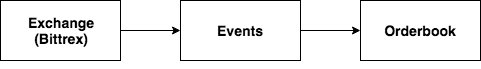
\includegraphics[width=8cm]{data-pipeline.png}
    }
    \caption{Data collection pipeline}
    \label{fig:data-pipeline}
\end{figure}

In this chapter, we will outline the details of the data collection process, and how this data can subsequently form a historical order book in order to serve as the historical data source for the match engine.
A sample period from the data set collected will then be investigated in order to find and visualize the properties of the market situation and behavior of the market participants.
The goal of the investigation is to find hypotheses which state why certain occurrences might be beneficial to consider for the purpose of limit order placement.
Thus, the findings serve as the basis for the feature construction process which determines the input for the learner.
Therefore, in the last section of this chapter, we will construct features which cover the stated hypotheses.
As a result, the features serve as the observed state that is to be evaluated by the reinforcement learning agents described in Chapter \ref{chap:setup}.

\section{Collection}
\label{sec:data-collection}

There are various ways to build a copy of a historical limit order book. However, the only way to rebuild a complete order book is by processing market \textit{events}, that is, every market update for a given ticker (trading pair, in our case USD/BTC).
There are three common types of events, all of which are initiated by a market participant (trader): \textit{order created}, \textit{order cancelled} or \textit{order filled} in the event that a market order crosses the spread and initiates a trade.

Our exchange of choice for collecting data is Bittrex\footnote{https://bittrex.com/} as the exchange provides a \textit{SignalR}\footnote{https://docs.microsoft.com/en-us/aspnet/signalr/overview/getting-started/introduction-to-signalr} (a library that abstracts \textit{HTTP} and \textit{WebSocket}) interface from which one can extract all status updates (events) from the market.
More specifically, an event in this either a buy or sell order, or a fill (e.g. trade).
Thus, we subscribe to \texttt{https://socket.bittrex.com/signalr} and filter the data field \texttt{M} for \texttt{updateExchangeState}.
The data type of the message contains the name of the trading pair and a nonce to identify the unique status update in up-counting order.
That is,
\begin{equation}
    StatusUpdate = \{name, nonce, buy_1,...buy_n, sell_1,...sell_n, fill_1,...fill_n\}
\end{equation}
, whereas $buy \in Order_{Limit}$, $sell \in Order_{Limit}$ (see Eq. \ref{eq:order-limit}) and $fill \in Trade$ (see Eq. \ref{eq:trade}).
With that said, the orders hold an additional field $type \in \{0,1,2\}$ which specifies whether it was a \textit{create}, \textit{cancel} or \textit{change} in the order, whereby the changes of orders are neglected in our setup as this function is rarely used by traders.

It is evident that multiple events can be sent within one status update message. 
We segment the status update into separate events with the same nonce, whereas each event expresses either a limit order of a side bid or ask or a filled order resulting in a trade,
\begin{equation}\label{eq:event-update}
    Event = \{name, nonce, type, isTrade, trade, isBid, order\}
\end{equation}
, whereas $isTrade \in \{0,1\}$ and $isBid \in \{0,1\}$ indicating whether the update contains an order or a trade. 
Consequently, $order \in Order_{Limit}$ and $trade \in Trade$.

\section{Order book generation}
\label{sec:data-generation}

The next step is to transform the events collected into an order book structure.
By chronologically iterating over the processed events (Eq. \ref{eq:event-update}), we create a new order book state (Eq. \ref{eq:order-book-state}) for each such event that has a consecutive time stamp.
During this iterative process, we follow the rules below, which ensure that the correct order book entries remain in future order book states.
Given the observed event, we act according to the type of the event:
\begin{description}
    \item[Order created:] an order book entry is added to the current state.
    \item[Order cancelled:] the amount of shares of the canceled order is subtracted from the entry in the current state with the corresponding price level.
    \item[Order filled:] the amount of shares traded is subtracted from the entry in the current state with the corresponding price level.
\end{description}
\hfill
\\
As a result, a \textit{list} of order book states is formed which constitutes a historical order book (Eq. \ref{eq:order-book}).
\textit{We acknowledge that a list representation is by no means the highest-performing method of implementing an order book, but for our purposes it is sufficient.}

\vfill

\section{Understanding the data set}
\label{sec:data-hypotheses}

We take a random period of the recorded data set, representing \textasciitilde10 minutes worth of event data, and try to extract essential information from either raw events or the order book that has been generated.
We first obtain an insight into the market situation with regard to some of the properties mentioned in Section \ref{sec:ob-characteristics} and understand how market participants place orders.
Our aim is then to find patterns of how market participants behave and how this may affect the market.
Subsequently, we formulate \textit{hypotheses} which propose why certain properties might be beneficial to the order placement process. The aim is to suggest which properties might be worth considering in the feature construction process.  However, we acknowledge that the observations gleaned are based on a random sample of a historical data set,
By no means does this method guarantee that the same observations are true for any order book.

Figure \ref{fig:data-price-movement} below shows the price movement of the sample period, indicating a movement from \$10,100 to \$10,030 and back within 10 minutes.

\begin{figure}[H]
    \centering
    \makebox[\linewidth]{
        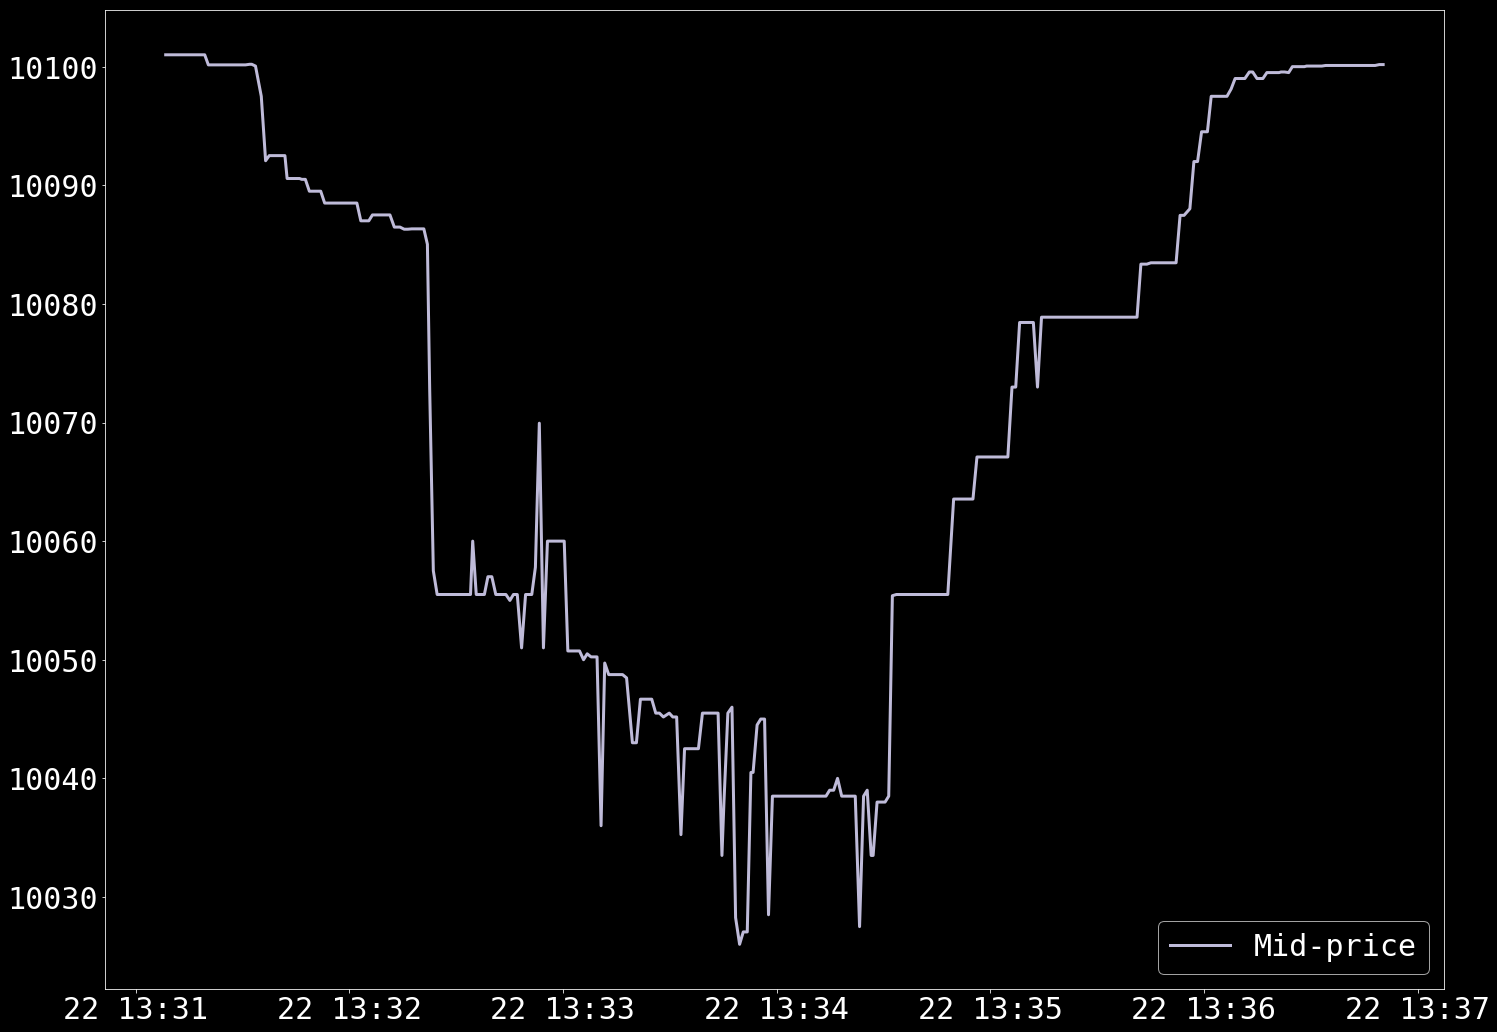
\includegraphics[width=12cm]{ob-price}
    }
    \caption{Price movement of sample data set}
    \label{fig:data-price-movement}
\end{figure}

\subsection{Importance of order prices}
\label{sec:data-hypthesis-order-price}

\begin{figure}[H]
    \centering
    \begin{subfigure}[b]{0.45\textwidth}
        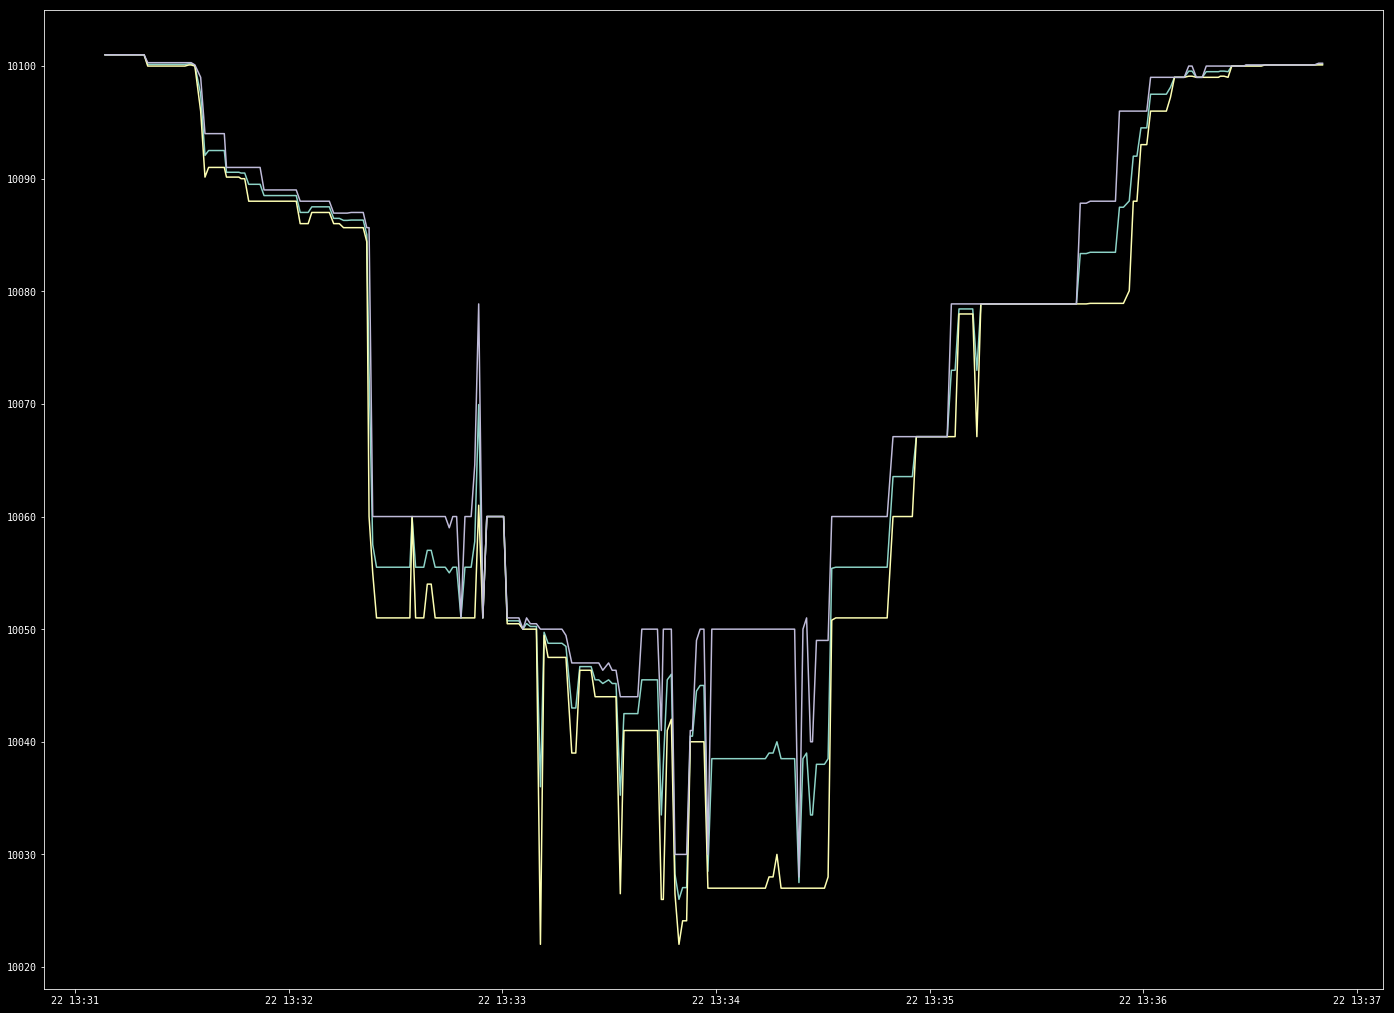
\includegraphics[width=\textwidth]{ob-ba-min}
        \caption{Best bid and best ask}
        \label{fig:ob-ba-min}
    \end{subfigure}
    ~ %add desired spacing between images, e. g. ~, \quad, \qquad, \hfill etc. 
    %(or a blank line to force the subfigure onto a new line)
    \begin{subfigure}[b]{0.45\textwidth}
        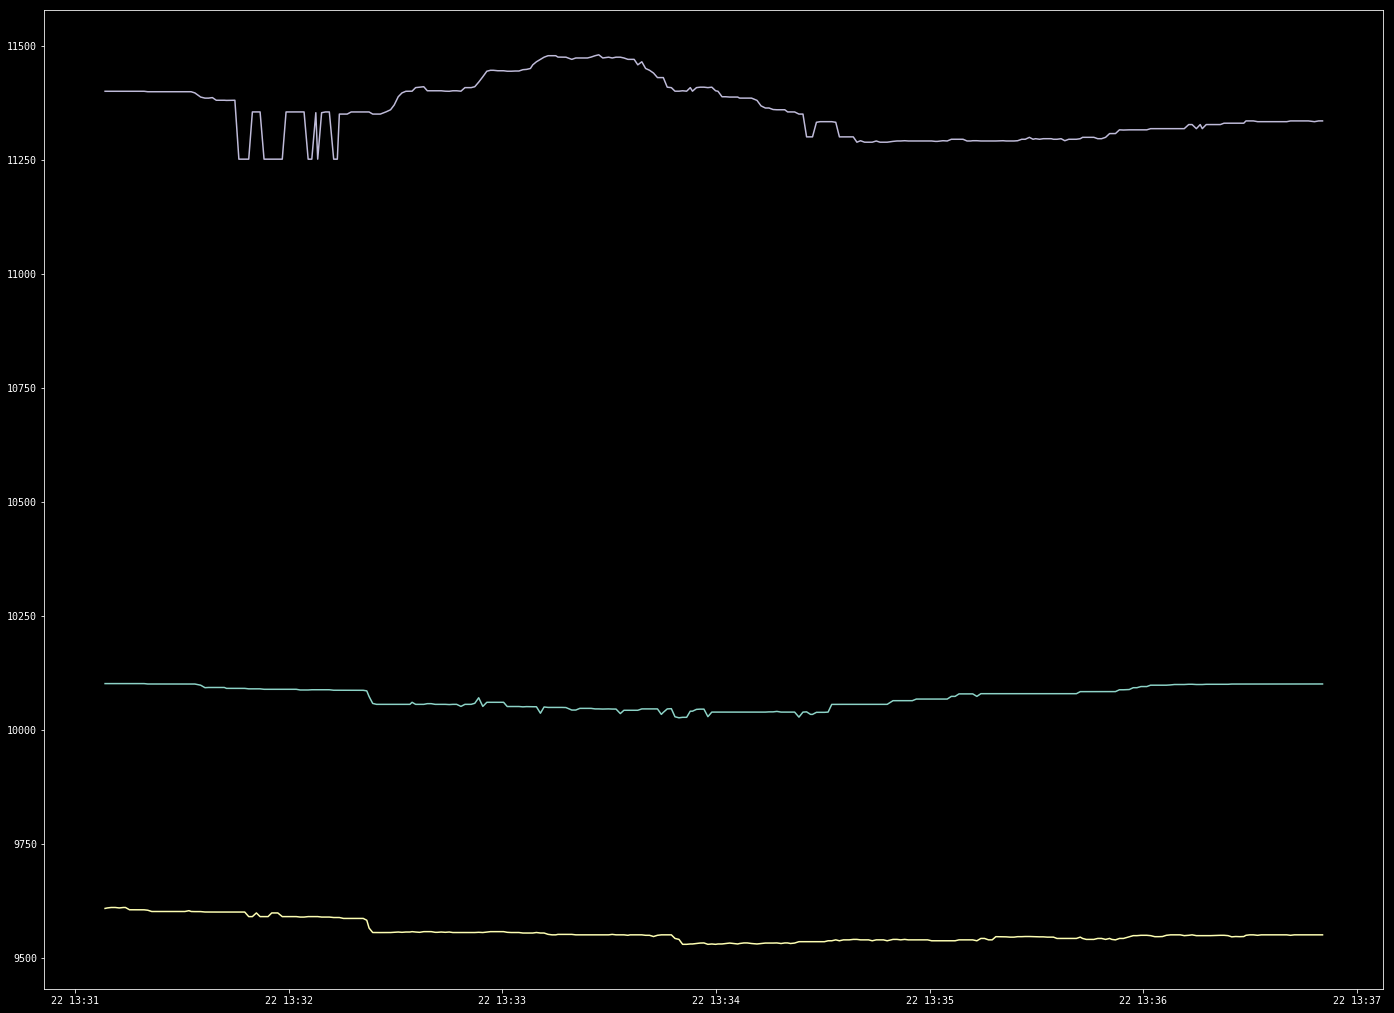
\includegraphics[width=\textwidth]{ob-ba-max}
        \caption{Deepest bid and deepest ask}
        \label{fig:ob-ba-max}
    \end{subfigure}
    \caption{USD/BTC price and bid/ask positions}\label{fig:animals}
\end{figure}

Next, we show the same price movement (cyan) but with the best bid (yellow) and ask (violet) (Figure \ref{fig:ob-ba-min}) and the deepest level of bid and ask (Figure \ref{fig:ob-ba-max}).
It is evident that the best bid and ask are close to the prices before and after the price dip, meaning the spread is narrow.
During the dip, the spread widens and is at times as large as \$25.
\\
\\
\textit{\textbf{Hypothesis:} participants post offerings close to the spread when the price is stable and start offering with a certain threshold from the spread during a price fall or rise.}
\\
\\
The orders placed at the deepest level on the buyer and seller side undergo a very interesting change.
Immediately before the the price dip, ask prices start to fluctuate as some participants cancel their listings and possibly others (trader cannot be associated as this is hidden information).
On the contrary, bid prices remain much more stable.
Likewise, during the fall and rise of the price, the ask price starts to increase at the deepest level of the seller side. 
This phenomenon is, at first glance, unexpected as one would expect the sell offers to be lowered as the price falls.
Knowing that the price rises shortly after, it becomes more evident that some sellers' intentions were to lure buyers by threatening them with higher sell listings.
The ask prices return to the level before the dip as soon as the price starts rising again.
\\
\\
\textit{\textbf{Hypothesis:} sellers lure buyers with higher listings during a price fall.}
%\\
%\begin{figure}[H]
%    \centering
%    \begin{subfigure}[b]{0.45\textwidth}
%        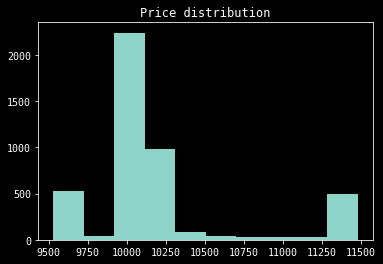
\includegraphics[width=\textwidth]{images/ob-price-bars}
%        \caption{Distribution of prices}
%        \label{fig:ob-price-dist-unfiltered}
%    \end{subfigure}
%    \begin{subfigure}[b]{0.45\textwidth}
%        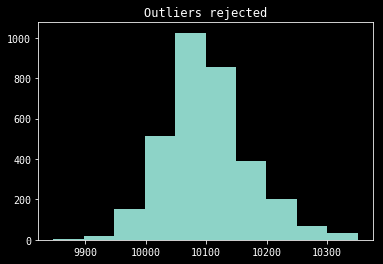
\includegraphics[width=\textwidth]{images/ob-price-bars-rejected}
%        \caption{Distribution of prices (filtered)}
%        \label{fig:ob-price-dist-filtered}
%    \end{subfigure}
%    \caption{Price distribution of events}\label{fig:price-distribution}
%\end{figure}
%
%Figure \ref{fig:ob-price-dist-unfiltered} shows the distribution of prices of all types of events (create, cancel, trade) within this data set.
%As can be seen, most of the events contain prices in the range of the traded price (see Figure \ref{fig:ob-price}) and significantly less below and above this range.
%However, the number of events increase with prices on both, the far end of the buyer and seller side, which supports the above stated hypothesis that orders deep in the book might in fact affect the price movement--even though they were not executed within the spectrum of this data set.
%We then filter events by rejecting outliers of their price $p$ according to standard deviation $\sigma$, $ |p_i - \overline{p}| < m * \sigma_{p} $, whereas $m=2$.
%As a result, Figure \ref{fig:ob-price-dist-filtered} shows the distribution of the prices from the filtered events, that follows a standard distribution.
%The mean lays at approximately \$10'100, the price level before and after the dip.
%\\
%\\
%\textit{\textbf{Hypothesis:} in case of a price dip (or raise) density estimation can be applied to find a more stable price level.}

\subsection{Importance of order volume}
\label{sec:data-hypthesis-order-volume}

It was shown that market participants position their offerings at different price levels as the asset price is moving due to trading.
The second variable in posting orders is the volume and we aim to determine whether or not this is a factor which is affected during the previously introduced price movement.

% \begin{figure}[H]
%     \centering
%     \begin{subfigure}[b]{0.45\textwidth}
%         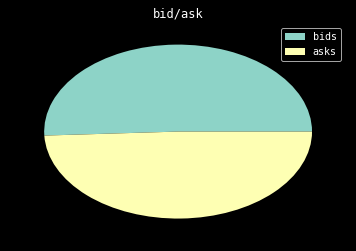
\includegraphics[width=\textwidth]{images/ob-ba-pie-all}
%         \caption{All events}
%         \label{fig:data-imbalance-events}
%     \end{subfigure}
%     \begin{subfigure}[b]{0.45\textwidth}
%         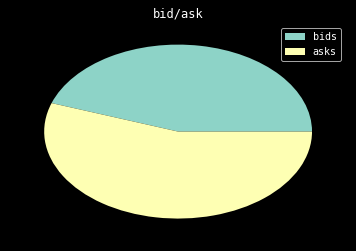
\includegraphics[width=\textwidth]{images/ob-ba-pie-trades}
%         \caption{Trades only}
%         \label{fig:data-imbalance-trades}
%     \end{subfigure}
%     \begin{subfigure}[b]{0.45\textwidth}
%         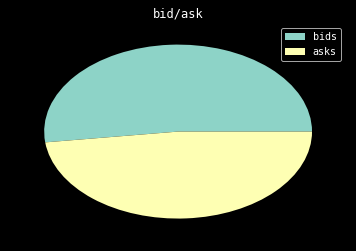
\includegraphics[width=\textwidth]{images/ob-ba-pie-created}
%         \caption{Create order only}
%         \label{fig:data-imbalance-creates}
%     \end{subfigure}
%     \begin{subfigure}[b]{0.45\textwidth}
%         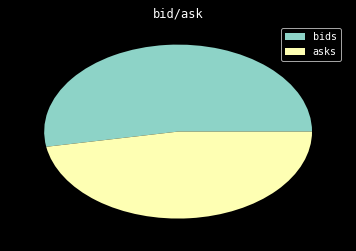
\includegraphics[width=\textwidth]{images/ob-ba-pie-cancelled}
%         \caption{Cancel orders only}
%         \label{fig:data-imbalance-cancels}
%     \end{subfigure}
%     \caption{Bid / Ask volume imbalance}\label{fig:data-imbalance}
% \end{figure}

\begin{table}[H]
\centering
\begin{tabular}{l|l|l|l|l|}
\cline{2-5}
& \textbf{All events} & \textbf{Trades only} & \textbf{Orders created} & \textbf{Orders cancelled} \\ \hline
\multicolumn{1}{|l|}{\textbf{Bids}} & 51\%                & 41\%                 & 54\%                    & 57\%                      \\ \hline
\multicolumn{1}{|l|}{\textbf{Asks}} & 49\%                & 59\%                 & 46\%                    & 43\%                      \\ \hline
\end{tabular}
\caption{Bid / Ask volume imbalance}
\label{tbl:data-imbalance}
\end{table}

Table \ref{tbl:data-imbalance} shows the (im-)balance of the volumes of bid and ask orders segmented into bids and asks of all events, including trades, creations and cancellations. 
It is evident that, even though the price moved significantly within the recorded time range, the entirety of the orders is well balanced between trades or orders on the bid side and the ask side.
For trades however, clearly more shares were sold than bought.
It is then evident that the market participants reacted on the sale of the asset by not only creating but also cancelling more buy than sell orders.
We take the last statement as an indication that the market participants may have responded to the price dip by cancelling their current buy orders and posting them deeper in the book (out of fear that the price might fall even further).
Interestingly, even though the price rose after the dip, not as much volume was used on creations and cancellations of orders on the seller side.
\\
\\
\textit{\textbf{Hypothesis:} imbalance of bids and asks of event types indicates future behaviour of participants.}

\subsection{Volume of orders and trades over time on the market price}
\label{sec:data-hypthesis-order-trade-volume-time}

So far, the volume was investigated as a sum of events over time.
In order to understand the behaviour of the participants in greater detail, a \textit{volume map} shall provide better insight into the single events occurred over time.

Figure \ref{fig:data-volmap-crated} shows the volume map of the orders which were created over the time span of the data set.
Hence, the x-axis represents the time stamp and the y-axis is the volume of the placed order.
For visibility reasons and since the majority of the orders have a small volume and fewer have large volume, the y-axis follows a log-scale.
Participants cannot be assigned to such an order, as the trader id is non-public information.
However, as we will see, one can determine some participants according to their behaviour.

\begin{figure}[H]
    \centering
    \makebox[\linewidth]{
        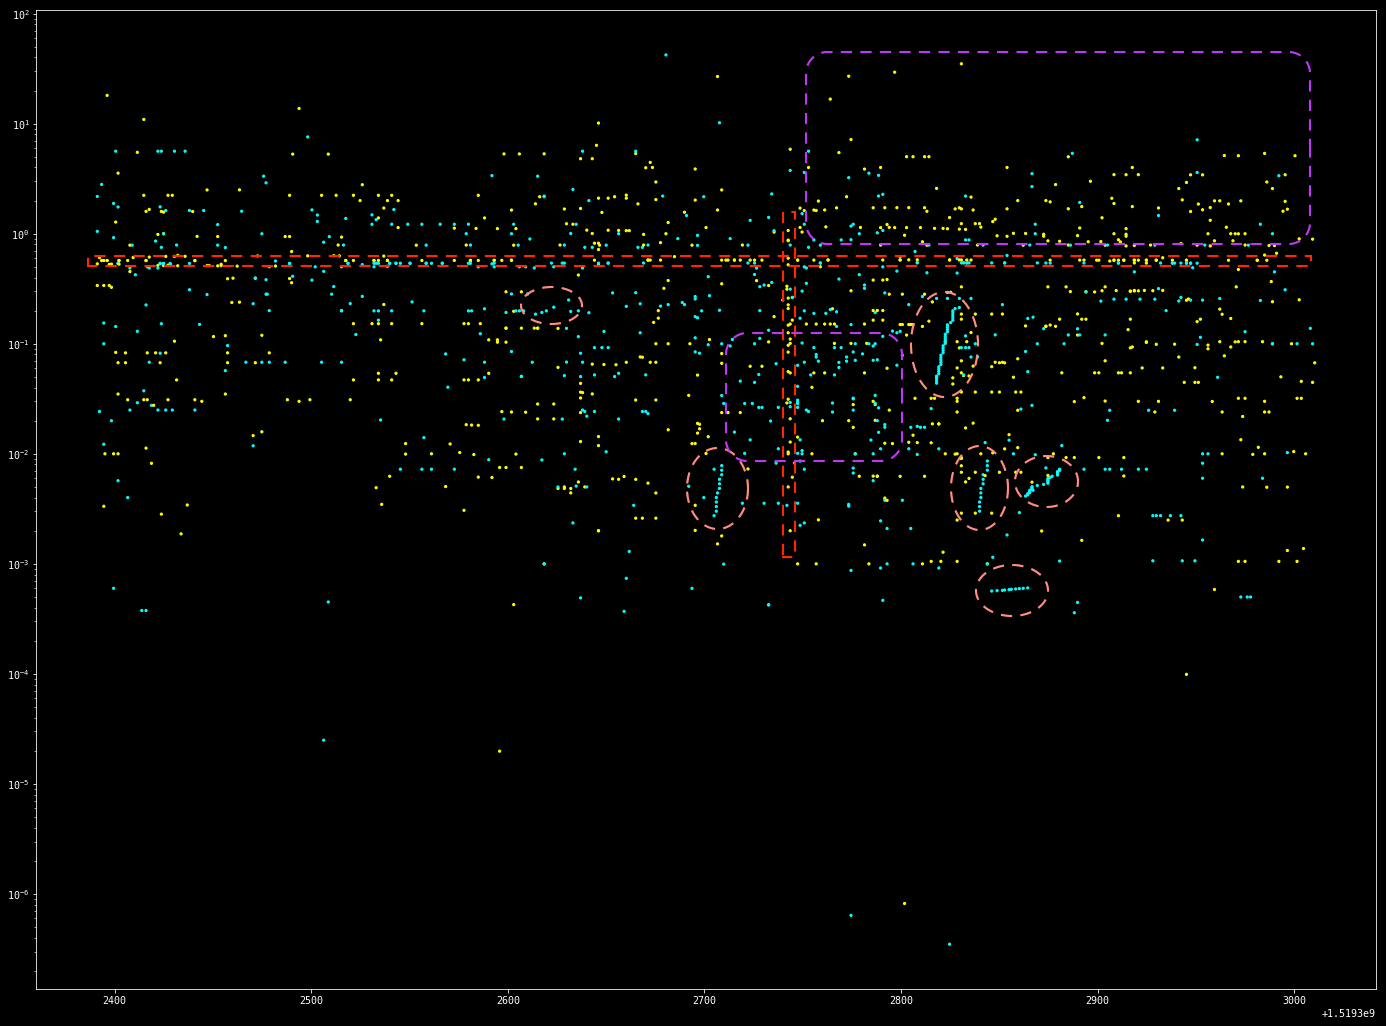
\includegraphics[width=14cm]{images/data-volmap-created}
    }
    \caption{Volume map of created bid (cyan) and ask (yellow) orders.}
    \label{fig:data-volmap-crated}
\end{figure}

What might not be obvious due to the log scaling is the fact that most of the orders were placed with volume between >0 and <0.5 and significantly less with larger volume.
Only a few orders had a volume greater than 10 BTC, meaning that most of the participants either are willing to buy and sell only small quantities or split their orders to minimize the market impact.

From a horizontal perspective, one can detect some orders of both sides, bids and asks, being listed with the same time interval.
Particularly evident is such a behaviour at the volume just below $10^0$.
This is likely one or multiple bots posting orders with the same volume and perhaps at a different price level.
Examples of this behaviour is marked with a red-dashed horizontal box.
A similar behaviour can be seen from a vertical perspective where one or more traders post orders at different price levels, with the same price segmentation.
This is market with a red-dashed vertical box.
Furthermore, a very distinctive pattern is when a trader posts orders within a short period of time but changing volume.
This might be evidence of someone splitting a larger order into small pieces and is marked with an orange-dashed circle.
Some refer to such a behaviour as \textit{buy-wall} (\textit{sell-wall} in case of an ask orders) and surprisingly, this behaviour appeared the most when before and during the price started rising again (compare time stamps from Figure \ref{fig:data-price-movement}).
Last but not least, examples of areas dominated by one particular order side (buy or sell) is marked with a purple box.

\begin{figure}[H]
    \centering
    \makebox[\linewidth]{
        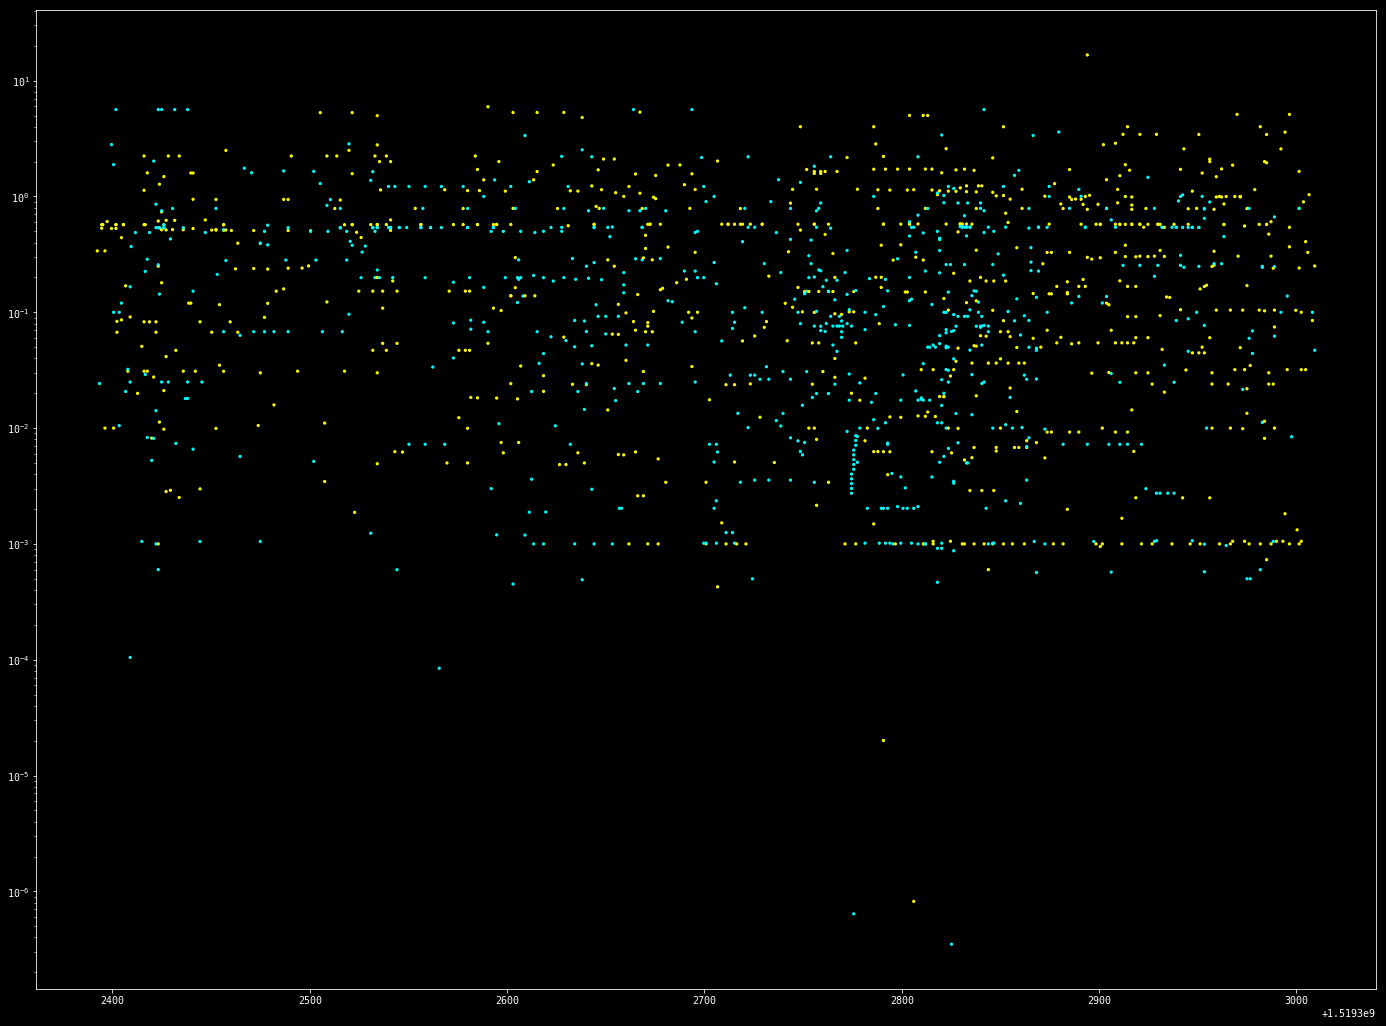
\includegraphics[width=14cm]{images/data-volmap-cancelled}
    }
    \caption{Volume map of cancelled bid (cyan) and ask (yellow) orders.}
    \label{fig:data-volmap-cancelled}
\end{figure}

It is to be expected that at least for some of the orders, which did not result in a trade, a cancellation followed.
Figure \ref{fig:data-volmap-cancelled} therefore shows the cancel orders posted by traders over time.

Continuous cancellations become especially evident at volume levels just below $10^0$ and $10^{-1}$, correlating with the continuous create orders appeared at the same price level above.
Hence, there is likely a trader following some strategy.
A cancellation of one of the created buy-walls is particularly evident at the same time stamp and with equal volumes as previously discovered.
Hence, making it more even more likely that the wall was created and cancelled by a single trader.
\vfill
\pagebreak

\begin{figure}[H]
    \centering
    \makebox[\linewidth]{
        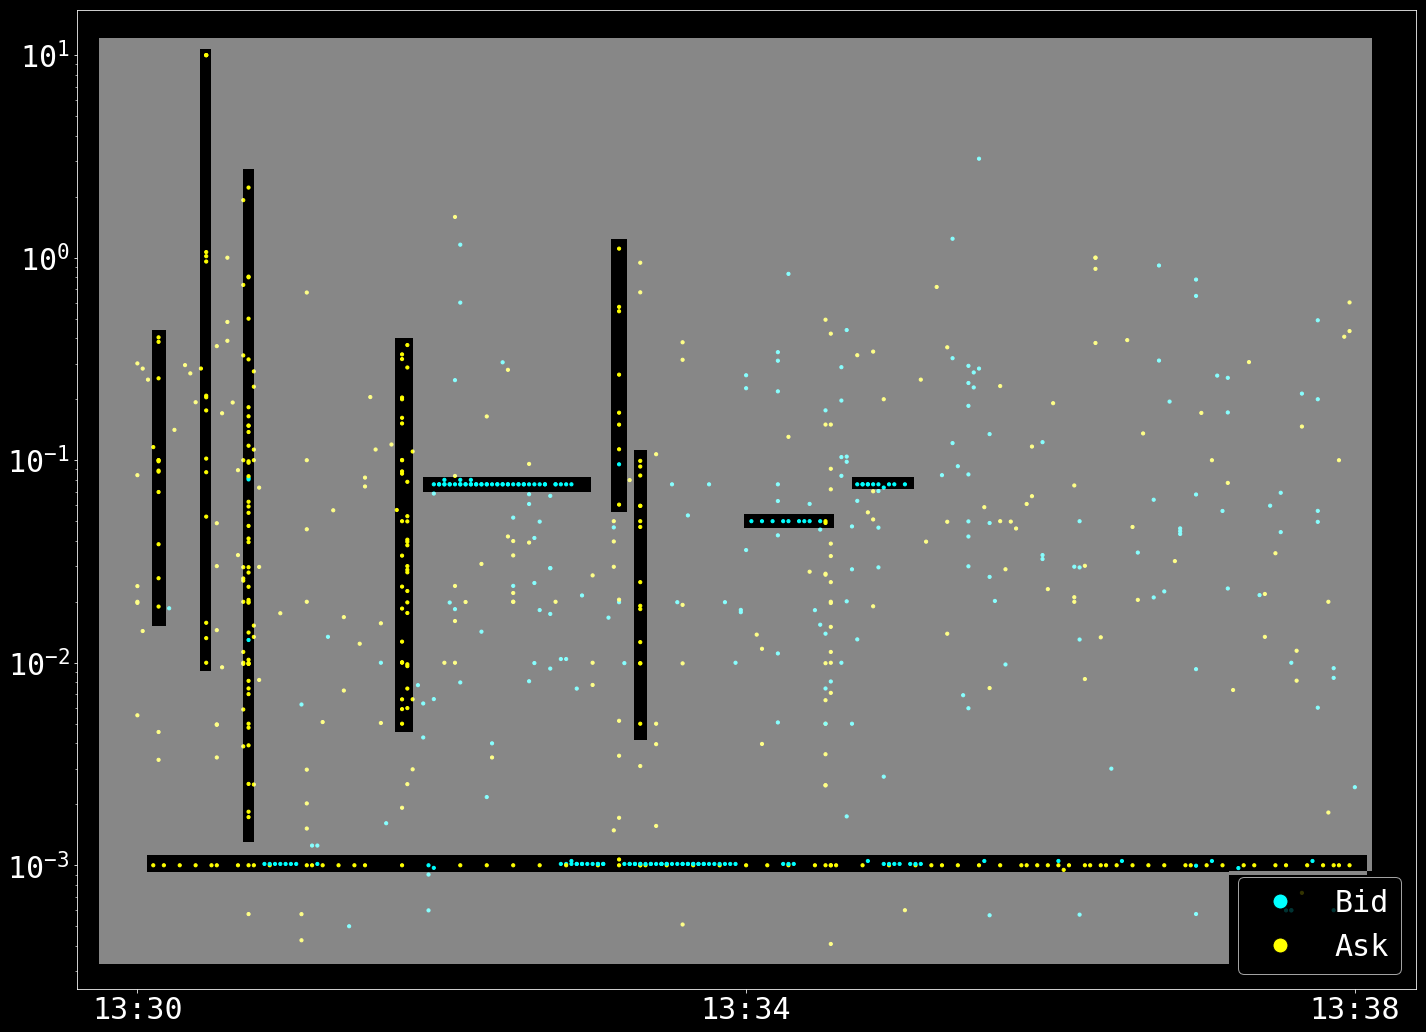
\includegraphics[width=14cm]{images/data-volmap-traded}
    }
    \caption{Volume map of trades initiated by a bid (cyan) or ask (yellow) order crossing the spread.}
    \label{fig:data-volmap-traded}
\end{figure}

So far only posted limit orders or their cancellation where observed.
Not all of those limit orders might have executed and resulted into a trade as there is always a market order required, initiated by one of the two parties involved in a trade.
Figure \ref{fig:data-volmap-traded} therefore illustrates the volume map of the actual trades occurred within this sample time range of the data set.

Immediately evident are the trades transacted with volume $10^{-3}$, with oftentimes identical time interval.
Additionally, an intensive series of consecutive sales occurred at the time when the price dipped.
After the dip, such sales are not present anymore.
Furthermore, intensive and immediate purchases are visible with various volume at some distinctive time stamps before and during the price fall.
We remember that there was one spike towards a higher price during the dip, and the time stamp of which correlates strongly to the purchases visible in this figure.
\\
\\
Various behavioural patterns have been observed by investigating events initiated by market participants over time.
For some, their impact on the market price is immediately obvious, for others it is hard to interpret by hand.
However, an attempt to find correlation between the behaviour of the events and the resulted trades with the application of learning techniques seems promising.
\\
\\
\textit{\textbf{Hypothesis:} patterns arising from posted volume in events determines future short-term trading behaviour which can be exploited in favour of order placement.}

\subsection{Impact of traded price and volume}
\label{sec:data-hypthesis-trade-price-volume}

The price levels and volume of events over time was investigated for each type in the previous subsections.
Patterns were found and a hypothesis was stated which encourages the various offerings of volume of an order to be an indicator of future behaviour of market participants, which eventually influences the market price and implicitly determines optimal order placement.
The next logical step is to investigate the sum of traded volume at a given point in time (as shown in Figure \ref{fig:data-volmap-traded}) in combination with the price the asset was traded for.

\begin{figure}[H]
    \centering
    \makebox[\linewidth]{
        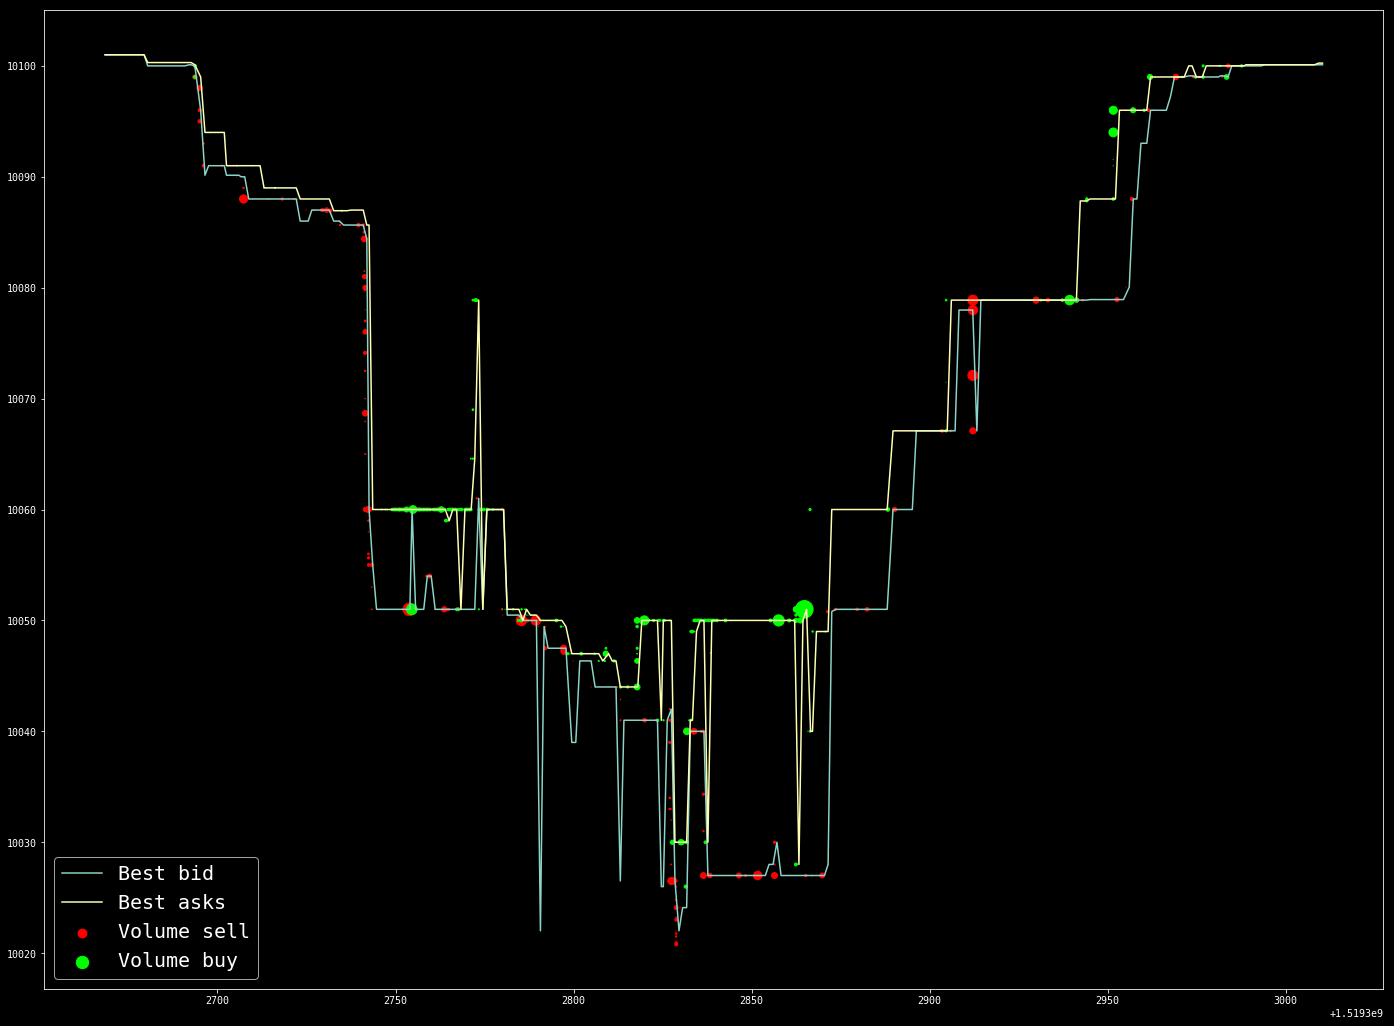
\includegraphics[width=14cm]{data-trade-volume}
    }
    \caption{Relation of trade volume to price movement.}
    \label{fig:data-trade-volume}
\end{figure}

Figure \ref{fig:data-trade-volume} illustrates the volumes of trades on both bid and ask side, which resulted in a buy or sell at a certain price.
The volume of these trades are illustrated as bubbles according to their size (e.g. traded volume) and price.
As is known, a buy appears when one crosses the spread towards the sellers side (ask) and a sell appears when crossing towards the buyer side (bid).
One can clearly see how buys are listed on the best ask price level and sells are listed on the best buy price level.
Before and during the dip sells appear consecutively, followed by a series of buy orders with low volume, which caused the short spike.
Interestingly, a rather large trade caused by a bid appeared shortly before the price started rising again.
Even though sellers confronted the market in the middle of the price rise, participants continued buying shortly after with approximately equal volume.
Concluding this observation it is evident that few trades with small volume caused a certain noise in the overall trend.
Multiple consecutive trades initiated one side or a single large the like, however, led the market price to move for substantially longer period of time.
\\
\\
\textit{\textbf{Hypothesis:} consecutive small or one large trade give an impulse that drives the market price up or down.}


\section{Feature construction}
\label{sec:feature-engineering}
The previous section demonstrated certain trading behaviours of the market participants in an order driven market, which ultimately determines the evolution of the limit order book. 
Hypotheses were laid out which give reasons to believe that the outcome in terms of a change in the order book constellation and price development can be related to aforementioned trading behaviour.
Consequently this implies that orders can be placed and filled at limit levels which result in a favourable price.
Therefore, the following subsections will introduce features that are derived from the previously collected (Section \ref{sec:data-collection}) and processed (Section \ref{sec:data-generation}) data and cover the assumptions stated in Section \ref{sec:data-hypotheses}.
Instead of hand-engineer features such as shown in \cite{nevmyvaka2006reinforcement, hwangdeep, fletcher2010multiple}, the aim of this project is to learn the knowledge directly from raw inputs, similar to what has been proven to be a successful method in the gaming sector\cite{mnih2013playing} and was recently applied to the trading context\cite{lu2017agent}.

\subsection{Feature: price and size of historical orders}
The order book was defined in Eq. \ref{eq:order-book} and generated in Section \ref{sec:data-generation} serves as the first feature.
More precisely for each sample at time $t$, we use $n$ order book entries (Eq.\ref{eq:order-book-entry}) of $m$ of the order book states (Eq. \ref{eq:order-book-state}) with time stamp $ts \le t$.
Therefore, as shown in Eq. \ref{eq:feature-bid-ask}, $s_{bidask} \in \mathbb{R^+}^{m\times2\times2n}$ is the state observed by a reinforcement learning agent.
The order book states are ordered such that $m$ is the closest to $t$.
The $n$ order book entries are closest to the spread whereas only the price $bp$ (respectively $ap$) and size $bs$ (respectively $as$) are considered.

\begin{equation}\label{eq:feature-bid-ask}
s_{bidask} =\begin{bmatrix}
{\displaystyle \begin{pmatrix}
bp_{11} & bs_{11}\\
bp_{12} & bs_{12}\\
\vdots  & \vdots \\
bp_{1n} & bs_{1n}\\
ap_{11} & as_{11}\\
ap_{12} & as_{12}\\
\vdots  & \vdots \\
ap_{1n} & as_{1n}
\end{pmatrix}} & \begin{pmatrix}
bp_{21} & bs_{21}\\
bp_{22} & bs_{22}\\
\vdots  & \vdots \\
bp_{2n} & bs_{2n}\\
ap_{21} & as_{21}\\
ap_{22} & as_{22}\\
\vdots  & \vdots \\
ap_{2n} & as_{2n}
\end{pmatrix} & \cdots  & \begin{pmatrix}
bp_{m1} & bs_{m1}\\
bp_{m2} & bs_{m2}\\
\vdots  & \vdots \\
bp_{mn} & bs_{mn}\\
ap_{m1} & as_{m1}\\
ap_{m2} & as_{m2}\\
\vdots  & \vdots \\
ap_{mn} & as_{mn}
\end{pmatrix}
\end{bmatrix} \ 
\end{equation}

Considering that the state will be observed by a deep learning agent, which makes use of a neural network, scaling of inputs will contribute to a faster learning process.
We therefore further apply normalization the the prices ($bp, ap$) with respect to the best ask price for each state, that is $ap_{i1}$.
Equivalently we normalize the sizes ($bs, as$) with respect to the size provided at the best ask $as_{i1}$.
While this method does not scale the values of prices and sizes within a predefined range, the values sill decrease significantly.
Furthermore, empirical observations show that the minimum and maximum of prices within a single order book state do not differ more than ~2\%, which determines the approximate scaling boundary.
\\
\\
This feature incorporates some of the previously stated hypotheses and therefore enables the learner to determine whether the statements were valid or not.
Particularly, the feature includes historical order prices (hypothesis \ref{sec:data-hypthesis-order-price}) their volume (hypothesis \ref{sec:data-hypthesis-order-volume} and partly \ref{sec:data-hypthesis-order-trade-volume-time}).
\\
\\
\todo[inline]{Might be unnecessary according to our talk.}
The question remains how large the window of $m$ order books states and the number of limit levels $n$ should be chosen.
The following observation provides an intuition about the parameters, however, this by no means aims to make an estimate how well the agent may perform under the consideration a certain parameter setup.

In order to reason about the impact of $n$ limit levels, we take the average of 100 evaluations whereas we take 1000 random order book states for which we measure the Shannon entropy\cite{shannon2001mathematical} for a range of 40 limit levels (maximum of what goes from collection) on the bid and ask side, applied to price and size.
The entropy therefore serves as an indicator of how much information can be gained for each limit level, derived from the their change in price and size for each state.

\begin{figure}[H]
    \centering
    \begin{subfigure}[b]{0.45\textwidth}
        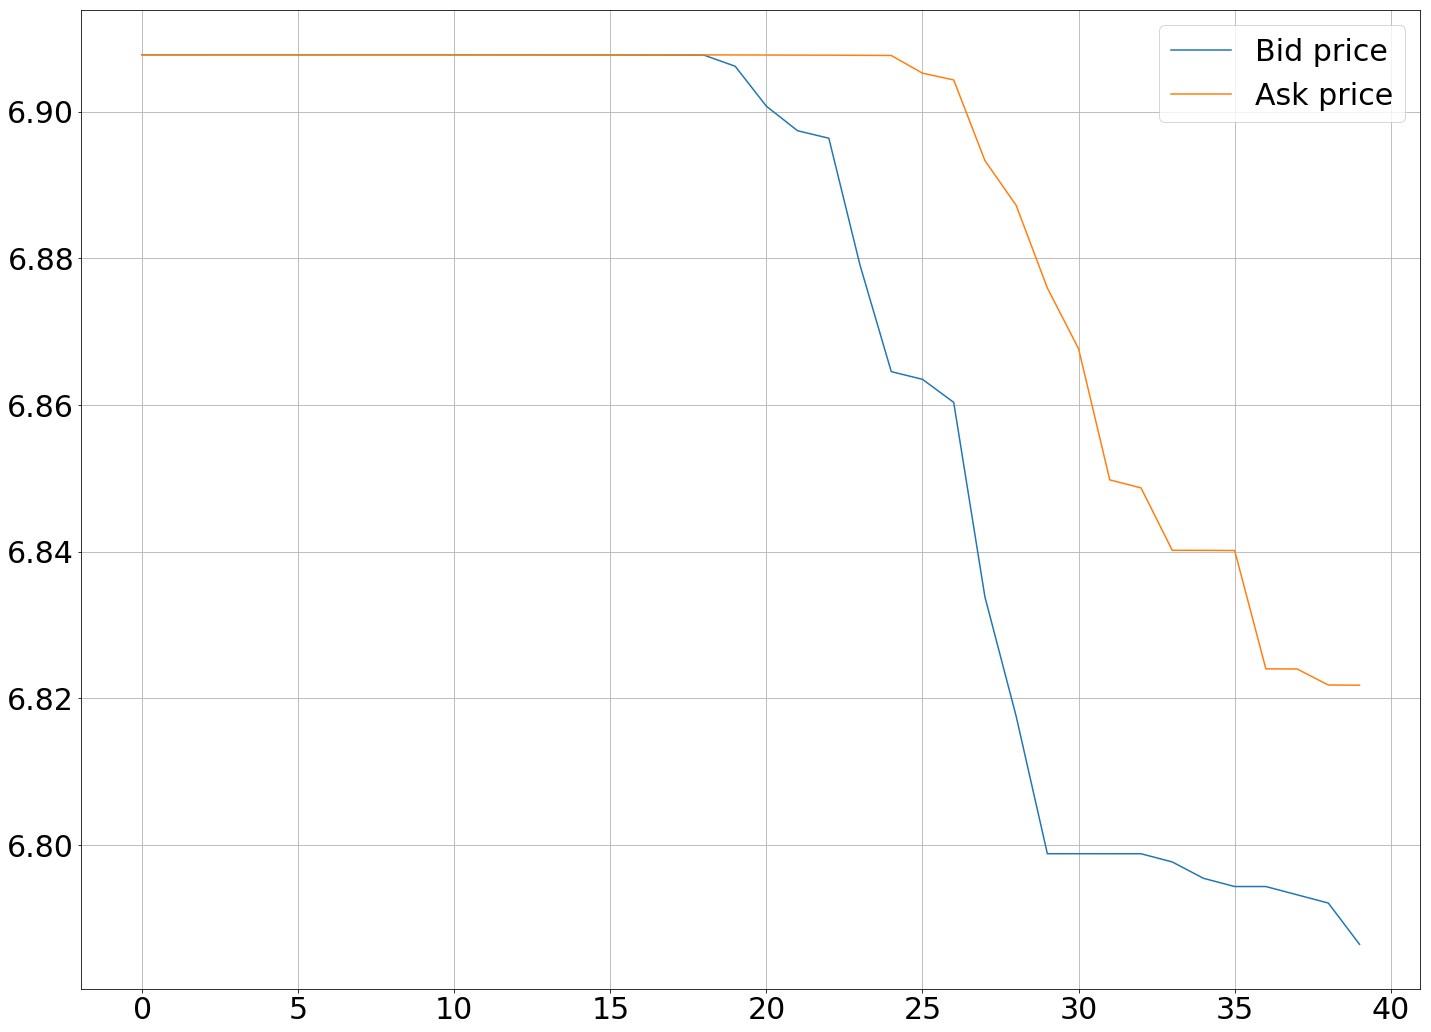
\includegraphics[width=\textwidth]{bidask-price-entropy}
        \caption{Entropy of order prices}
        \label{fig:bidask-price-entropy}
    \end{subfigure}
    \begin{subfigure}[b]{0.45\textwidth}
        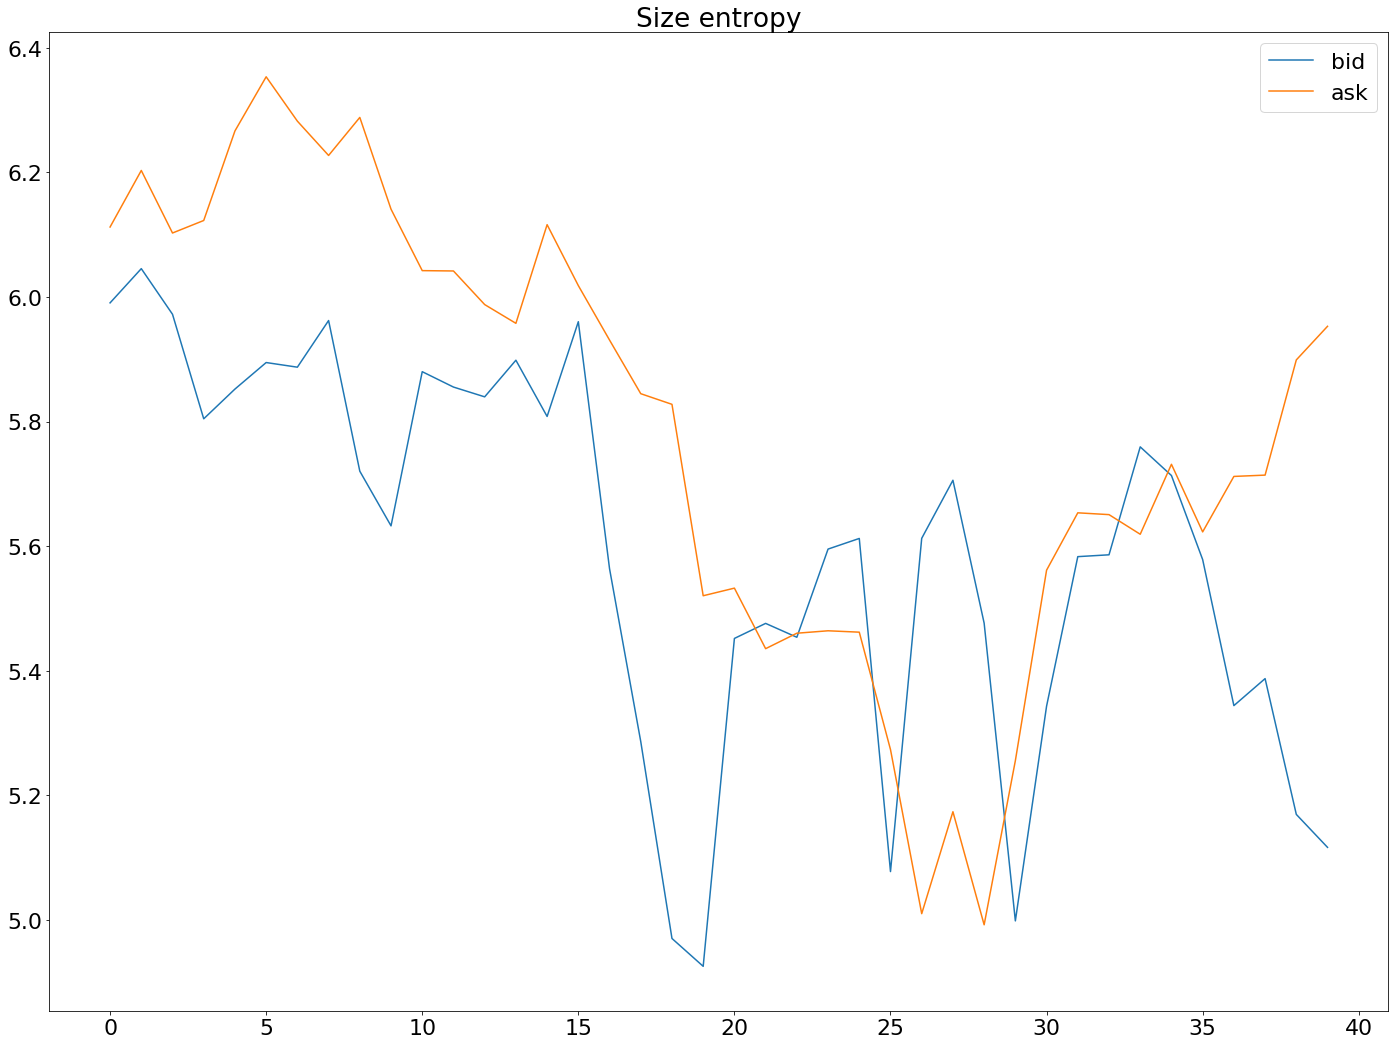
\includegraphics[width=\textwidth]{bidask-size-entropy}
        \caption{Entropy of order sizes}
        \label{fig:bidask-size-entropy}
    \end{subfigure}
    \caption{Entropy measured for 40 limit levels}\label{fig:bidask-entropy}
\end{figure}

It is noticeable that the entropy remains high regarding the prices for for limit levels 0-30 on both, bid and ask side, as shown in Figure \ref{fig:bidask-price-entropy}. 
The price becomes slightly more constant for limit levels $>30$. 
The entropy for order sizes, as shown in Figure \ref{fig:bidask-size-entropy}, drop after 20 limit levels, which indicates that the accumulated order size deep in the book is more constant. 
We therefore suggest to consider at least 30 limit levels of the bid-ask feature.

\begin{figure}[H]
    \centering
    \begin{subfigure}[b]{0.45\textwidth}
        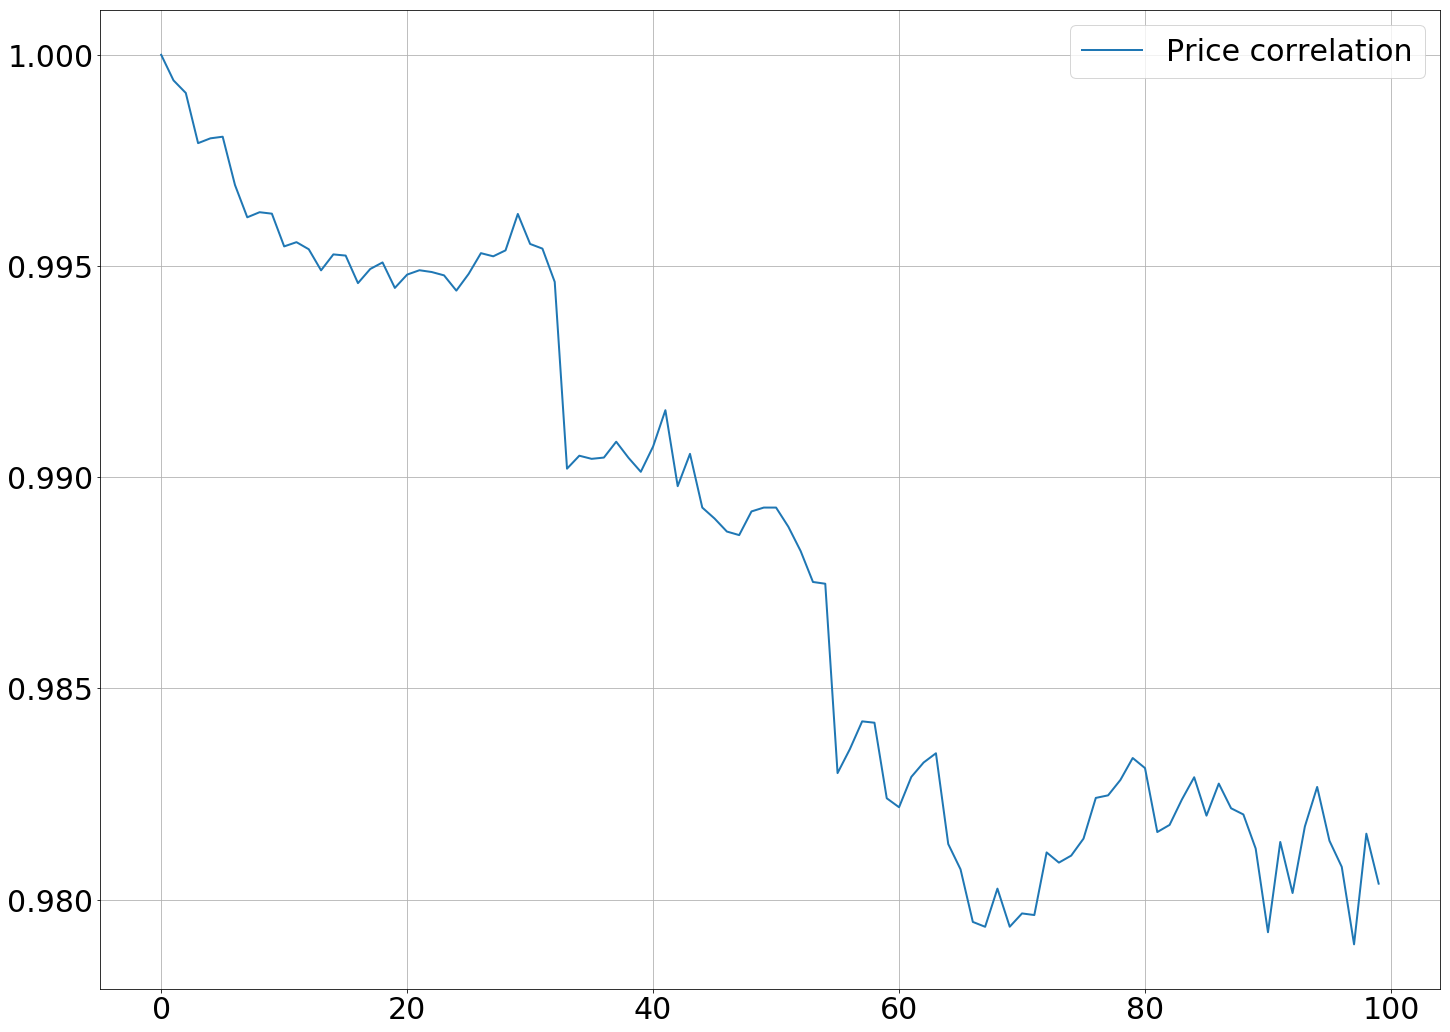
\includegraphics[width=\textwidth]{bidask-price-correlation}
        \caption{Correlation of order prices}
        \label{fig:bidask-price-correlation}
    \end{subfigure}
    \begin{subfigure}[b]{0.45\textwidth}
        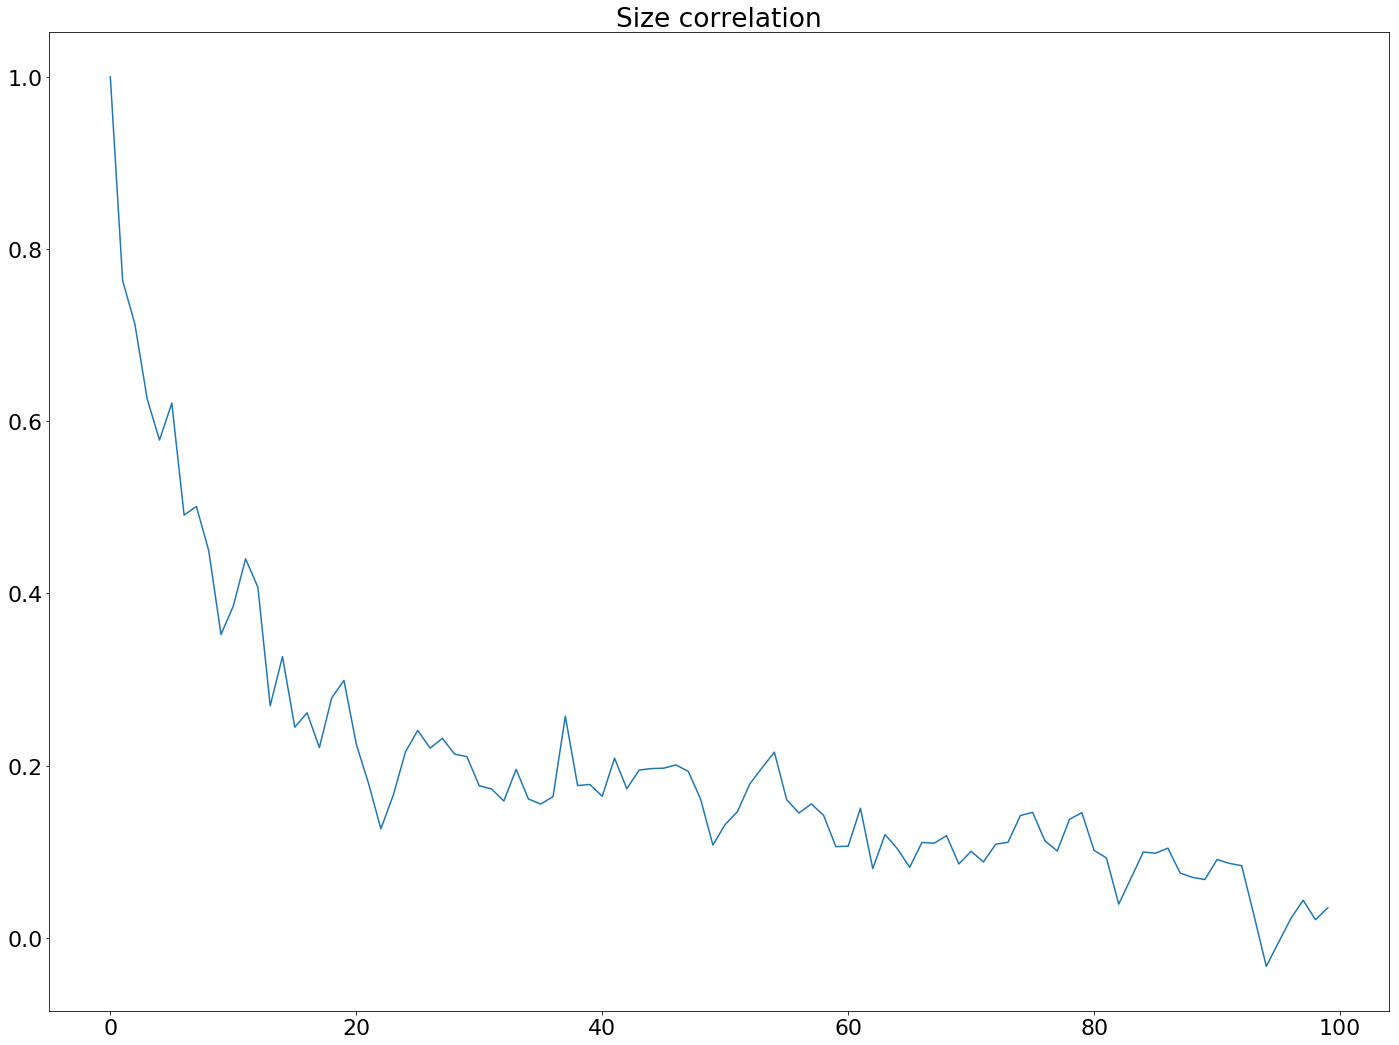
\includegraphics[width=\textwidth]{bidask-size-correlation}
        \caption{Correlation of order sizes}
        \label{fig:bidask-size-correlation}
    \end{subfigure}
    \caption{Correlation measured for 100 order book states}\label{fig:bidask-correlation}
\end{figure}

After having a brief understanding of how limit levels $n$ affect order prices and sizes, we try to make a statement about how order book states are related to the most recent state.
More precisely, we determine the correlation of the order prices and sizes from the previous $m$ states to the most recent order book state.
We take the average of 100 evaluations whereas we take a single order book state at time $t$ and a sequence of 100 previous order book states for each of which we measure the Shannon entropy\cite{shannon2001mathematical} to the state at $t$, whereas $n=40$ (maximum).
As can be seen in Figure \ref{fig:bidask-price-correlation}, the correlation of the price positions drop rapidly, however the effective change is not significant, indicating that the price changes are noticeable but overall do not differ much.
Order book states which lay more than 40 states in the past are slightly less correlated to the current state.
The correlation of order sizes, as shown in Figure \ref{fig:bidask-size-correlation} drops more rapid and to a much greater extent than the order prices.
This indicates that traders choose a broad range of order sizes.
As a result, a window size of order book states $m$ greater than 40 states is suggested to benefit from price differences within the feature.

\subsection{Feature: price and size of historical trades}
The previous feature provides information to the learner in order to reason about the hypotheses which are derived from order placed and cancelled.
In order to reason about whether or not trade events can provide a positive learning effect to the agent to optimize order placement, we construct a feature that covers the hypotheses \ref{sec:data-hypthesis-trade-price-volume} and partially \ref{sec:data-hypthesis-order-trade-volume-time} as follows.
A $Trade$ (Eq. \ref{eq:trade}) carries an order side $os$, a quantity $q$ and a price $p$.
Similar to the previous feature, in this feature we take $n$ trades into consideration, which occurred prior the time of the order placement.
More precisely, the feature is generated at some time $t$, when an order is placed, and therefore the time stamp $ts$ of the historical trades must satisfy $ts \leq t$.
\\
\\
A straightforward approach would be to construct the feature $s_{trade}$ as,
\begin{equation}
    s_{trade} =\begin{pmatrix}
        p_1 & q_1 & os_1 \\
        p_2 & q_2 & os_2 \\
        \vdots & \vdots & \vdots\\
        p_n & q_n & os_n \\
    \end{pmatrix}
    \ \forall \ p, q, os, ts \in Trade
\end{equation}, whereas $ts_n - ts_1 \leq m$.
However, trades do not occur in fixed time intervals and therefore causes the length of the vector to vary.
We therefore calculate the time difference $\Delta{ts}$ of each historical trade to the subsequent historical trade.
For the most recent historical trade, the time difference is measured to the time of the order placement $t$.
That is,
\begin{equation}
    \Delta{ts}_i = \begin{cases}
    t - ts_i &\text{if i = 1}\\
    ts_{i+1} - ts_i &\text{otherwise}
    \end{cases}
\end{equation}

As a result we can redefine the feature $s_{trade}$, that is used by the learner as observation state, as,
\begin{equation}
    s_{trade} =\begin{pmatrix}
        \Delta{ts_1} & p_1 & q_1 & os_1 \\
        \Delta{ts_2} & p_2 & q_2 & os_2 \\
        \vdots & \vdots & \vdots & \vdots\\
        \Delta{ts_n} & p_n & q_n & os_n \\
    \end{pmatrix}
    \ \forall \ p, q, os, ts \in Trade
\end{equation}
\hfill
\\
\\
In addition, the feature is normalized whereby the prices are divided by the market price $p_t$ and the quantities are divided by the size of the order $q_t$ which is about to be placed at time $t$.
As a result we constructed a feature vector of length $n$ (number of trades) that contains information about the price, order side and quantity of historical trades as well as their order of occurrence.

\section{Conclusion}

Event data was collected from a crypto-currency exchange and a limit order book was reconstructed thereof.
The limit order book serves as the historical data set and source for the match engine in order to simulate order placement. 
Subsequently the price chart as the result of the generated order book was shown and an investigation of the underlying event data was proceeded.
Patterns were found which give insight in how market participants positioned their offerings with respect to price and size.
It was shown that the price movement was likely due to (1) an imbalance in bid and ask orders; (2) a distinctive way of posting or cancelling orders; and (3) consecutive or impulsive trades.
These findings were incorporated within the feature engineering process, which resulted in two features that can be used by the reinforcement learning agents.